Refer to the data on snow storms in Exercise 3.20.
\begin{enumerate}[label= (\alph*)]
    \item Find a 95\% confidence region for the mean vector after taking an appropriate transformation.
    
    In Exercise 4.41, the multivariate transformations found were $(\hat{\lambda}_{1}, \hat{\lambda}_{2}) = (0.2349, -0.6376)$. I rounded these off to 0.25 and -0.70, respectively. The $100(1-\alpha)$\% confidence region, as stated on page 221, is the ellipsoid determined by all $\bm{\mu}$, such that,

    \[
        n {(\bar{\textbf{x}} - \bm{\mu})}^{\prime}
        \textbf{S}^{-1}
        (\bar{\textbf{x}} - \bm{\mu})
        \leq
        \frac{(n-1)p}{n-p}
        F_{p, n-p}(\alpha)
    \]

    \begin{figure}[H]
        \centering
        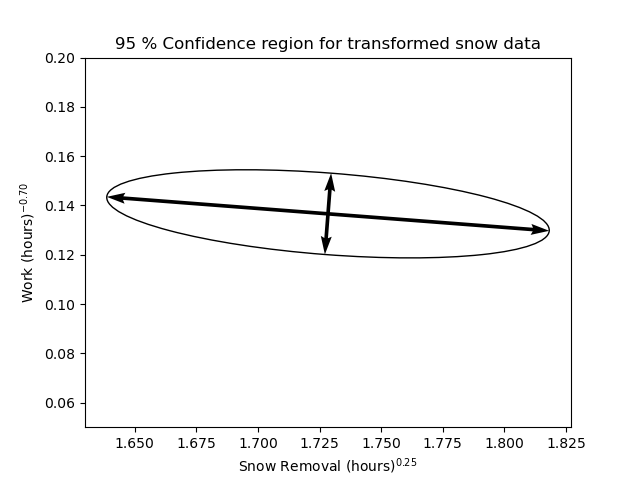
\includegraphics[scale=0.65]{./python/chapter-5/Question-5-31-a-Confidence-Region.png}
    \end{figure}

    \item On the same scale, find the 95\% Bonferroni confidence intervals for the two component means.
    \[
        \bar{x}_{i}
        \pm
        t_{n-1}
        \left(\frac{\alpha}{2m}\right)
        \sqrt{
            \frac{
                    s_{ii}
                }{
                    n
                }
            }
    \]

    \[
        \begin{NiceArray}{rrrr}
            1.73 \pm 2.39 \frac{\sqrt{0.0282}}{\sqrt{25}} & \text{contains }\mu_{1} & \text{ or } & 1.65 \leq \mu_{1} \leq 1.81 \\
            0.14 \pm 2.39 \frac{\sqrt{0.0011}}{\sqrt{25}} & \text{contains }\mu_{2} & \text{ or } & 0.12 \leq \mu_{2} \leq 0.15
        \end{NiceArray}
    \]
\end{enumerate}